\documentclass{beamer}
\usepackage{pgfpages}
%\setbeameroption{show notes on second screen=left} %enable for notes
\usepackage{graphicx}
\usepackage{xcolor}
\usepackage{listings}
%\usepackage{transparent}
\usepackage{hyperref}
\lstset{language=python,frame=single}
\usepackage{verbatim}
%\usepackage{apacite}
\usepackage[longnamesfirst]{natbib}
\usepackage{subcaption}
\usepackage{amsmath}
\usepackage{relsize}
\usepackage{appendixnumberbeamer}
\usepackage{xparse}
\usepackage{multimedia}
\usepackage{xcolor}
\usepackage[normalem]{ulem}
\usepackage{tikz}
\usetikzlibrary{matrix,backgrounds}
\usetikzlibrary{positioning}
\usetikzlibrary{shapes,arrows}
\usetikzlibrary{positioning}

\tikzset{onslide/.code args={<#1>#2}{%
  \only<#1>{\pgfkeysalso{#2}} 
}}

\tikzstyle{block} = [rectangle, draw, fill=red!20!blue!10, 
    text width=5em, text centered, rounded corners, minimum height=4em]
\tikzstyle{netnode} = [circle, draw, very thick, inner sep=0pt, minimum size=0.5cm] 
\tikzstyle{relunode} = [rectangle, draw, very thick, inner sep=0pt, minimum size=0.5cm] 
    
\tikzstyle{line} = [draw, line width=1.5pt, -latex']

\pgfdeclarelayer{background}
\pgfsetlayers{background,main}

\pgfdeclarelayer{myback}
\pgfsetlayers{myback,background,main}

\usetheme[numbering=fraction]{metropolis}

\newcommand\blfootnote[1]{%
  \begingroup
  \renewcommand\thefootnote{}\footnote{#1}%
  \addtocounter{footnote}{-1}%
  \endgroup
}
\renewcommand*\footnoterule{}
%%\AtBeginSection[]
%%{
%%  \begin{frame}
%%    \frametitle{Table of Contents}
%%    \tableofcontents[currentsection]
%%  \end{frame}
%%}

\begin{document}

\title{}
\author{Andrew Lampinen}
\date{FriSem, 5/11/2018}
\frame{\titlepage}

\begin{frame}[standout]
How do people learn so rapidly? \par
\only<2->{Claim: Transfer.}
\end{frame}


\begin{frame}{Transfer across domains}
Not a new idea: e.g. \cite{Gick1980, Gentner2003}
\uncover<2>{
\only<-2>{
\begin{figure}
\centering
\begin{subfigure}{0.4\textwidth}
\includegraphics[width=\textwidth]{figures/chess_cropped.jpg}
\end{subfigure}%
\begin{subfigure}{0.4\textwidth}
\includegraphics[width=\textwidth]{figures/go.jpg}
\end{subfigure}\\
\begin{subfigure}{0.4\textwidth}
\includegraphics[width=\textwidth]{figures/math.jpg}
\end{subfigure}%
\begin{subfigure}{0.4\textwidth}
\includegraphics[width=\textwidth]{figures/piano.jpg}
\end{subfigure}%
\end{figure}
}
}
\only<3>{
\begin{figure}
\centering
\includegraphics[width=0.8\textwidth]{figures/category_theory.jpg}
\end{figure}
}
\uncover<2->{
\scriptsize
\citep{Lampinen2017a, Hansen2017}
}
\note{There are deep relationships among the tasks we do -- some are superficially obvious, like Go and Chess, and some are less so, like the mathematical structures underlying music or the fact that we use language to talk about all these domains.\par
Of particular interest to me is deep isomorphisms between mathematical domains, and this is actually one of the things that inspired Gick \& Holyoak.}
\end{frame}

\begin{frame}{Criticism?}
However, this perspective has been criticized!\par
\begin{itemize}
\item<2-> ``Significant transfer is probably rare and accounts for very little human behavior.'' \citep{Detterman1993}
\item<3-> From FriSem last year: 
\begin{figure}
\centering
\includegraphics[width=0.4\textwidth]{figures/perspectives_on_transfer.png}
\end{figure}
\end{itemize}
\note{Detterman: ``We generally do what we have learned to do and no more.'' Experimental manipulations in transfer experiments ``have the subtlety of a baseball bat.''\par
Observation from FriSem last year: there is a correlation between the speed of transfer being sought and how important they think it is.}
\end{frame}

\begin{frame}{Transfer speed}
\vspace{1.5em}
What do I mean by ``fast'' and ``slow?''\par
\uncover<2->{
\begin{center}
\begin{table}
\begin{tabular}{|c|c|}
\hline
Fast & Slow \\
\hline
\parbox{0.45\textwidth}{
    \begin{itemize}
    \item<2-> one (or a few) examples explicitly shown
    \item<3-> transfer requires explicit awareness of analogy\\[5em]
    \end{itemize}
}
&
\parbox{0.45\textwidth}{
    \begin{itemize}
    \item<2-> learning through many interactions
    \item<3-> {transfer may or may not be explicit}%
               %%\only<4>{\color{red}transfer may or may not be explicit}}
    \item<4-> may take developmental time, or at least a long experiment!
    \end{itemize}
}\\ \hline
\end{tabular}
\end{table}
}
\vspace{1.5em}
\note{E.g. being told about the rules of chess and then seeing if that helps you play go, vs. playing many games of chess and go and seeing if one helps the other}
\end{center}
{
\scriptsize
\citep{Lampinen2017a}
}
\end{frame}

\begin{frame}[standout]
Slow transfer between tasks is important.
\end{frame}

\begin{frame}{Abstraction as a kind of transfer}
We often progress from procedural to more formal knowledge, e.g. in mathematics:
\begin{figure}
\centering
\begin{tikzpicture}
\node (img1) {\includegraphics[width=0.33\textwidth]{figures/multiplication_procedural_smaller.png}};
\only<2->{
\node (img2) at ([yshift=-2em]img1.east) {\includegraphics[width=0.33\textwidth]{figures/factoring_polynomial_worksheet.png}};
}
\only<3->{
\node (img3) at ([yshift=-3em]img2.east) {\includegraphics[width=0.5\textwidth]{figures/prime_ideals.png}};
}
\end{tikzpicture}
\end{figure}
\uncover<4>{This can be seen as a kind of transfer!}
\note{worksheetfun.com\par
Less abstract and more abstract reasoning can be seen as partially distinct tasks that share some common structure. There are different ways that procedural knowledge could support more formal, setting up representations and intuitions, having examples to reason over, ...}
\end{frame}

\begin{frame}[standout]
Abstraction is one type of task where we might look for transfer.
\end{frame}

\begin{frame}<-8>[label=phenomena]
\frametitle<-8>{A diagram of potential phenomena of interest}
\frametitle<9>{Abstractions?}
\begin{figure}
\centering
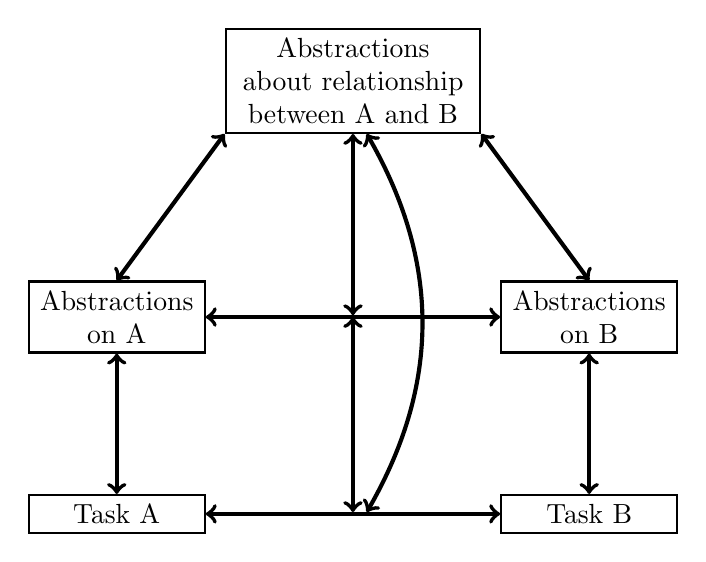
\begin{tikzpicture}[auto] %% TODO? highlighting
\node [rectangle, draw, thick, text width=2cm, align=center, onslide={<9>,{opacity=0.2}}] (A) at (-3, 0) {Task A}; 
\node [rectangle, draw, thick, text width=2cm, align=center, onslide={<9>,{opacity=0.2}}] (B) at (3, 0) {Task B}; 
\uncover<2->{
\path [line, <->, onslide={<9>,{opacity=0.2}}] (A.east) to node (proctrans) {} (B.west); 
}
\uncover<3->{
\node [rectangle, draw, thick, text width=2cm, align=center] (Aabs) at (-3, 2.5) {Abstractions on A}; 
\node [rectangle, draw, thick, text width=2cm, align=center] (Babs) at (3, 2.5) {Abstractions on B}; 
\path [line, <->, onslide={<9>,{opacity=0.2}}] (A.north) to  node (Atrans) {}(Aabs.south); 
\path [line, <->, onslide={<9>,{opacity=0.2}}] (B.north) to node (Btrans) {} (Babs.south); 
}
\uncover<4->{
\path [line, <->, onslide={<9>,{opacity=0.2}}] (Aabs.east) to node (abstrans) {} (Babs.west); 
}
\uncover<5->{
\path [line, <->, onslide={<9>,{opacity=0.2}}] ([yshift=-0.75em]proctrans.north) to node (procabstrans) {} (abstrans.south); 
}
\uncover<6->{
\node [rectangle, draw, thick, text width=3cm, align=center] (ABabs) at (0, 5.5) {Abstractions about relationship between A and B}; 
}
\uncover<7->{
\path [line, <->, onslide={<9>,{opacity=0.2}}] (Aabs.north) to  (ABabs.south west); 
\path [line, <->, onslide={<9>,{opacity=0.2}}] (Babs.north) to  (ABabs.south east); 
}
\uncover<8->{
\path [line, <->, onslide={<9>,{opacity=0.2}}] ([yshift=-0.75em]abstrans.north) to(ABabs.south); 
\path [line, <->, bend right, onslide={<9>,{opacity=0.2}}] ([xshift=0.5em, yshift=-0.75em]proctrans.north) to([xshift=0.5em]ABabs.south); 
}

\end{tikzpicture}
\end{figure}

\end{frame}

\section{Experiment design}

\begin{frame}{Experiment design}
\only<3->{
\vspace{-1em}
}
\begin{figure}
\centering
\begin{tikzpicture}[auto] 
\node (time00) at (-2, -1) {};
\node (time01) at (5, -1) {};
\node [rectangle, draw, thick, text width=2cm, minimum height=1.5cm, align=center ] (A) at (0, 0) {Task A}; 
\node [rectangle, draw, thick, text width=2cm, minimum height=1.5cm, align=center] (B) at (3, 0) {Task B}; 
\path [line, ->] (time00) to (time01); 

\only<2->{
\node (sess1) at (-2.5, 0) {\bf Day 1};

\node (sess2) at (-2.5, -2.5) {\bf Day 2};
\node (time10) at (-2, -3.5) {};
\node (time11) at (5, -3.5) {};
\node [rectangle, draw, thick, text width=2cm, minimum height=1.5cm, align=center ] (A1) at (0, -2.5) {Task A}; 
\node [rectangle, draw, thick, text width=2cm, minimum height=1.5cm, align=center] (B1) at (3, -2.5) {Task B}; 
\path [line, ->] (time10) to (time11); 

\node (sess1) at (-2.5, -5) {\bf Day 3};
\node (time20) at (-2, -6) {};
\node (time21) at (5, -6) {};
\node [rectangle, draw, thick, text width=2cm, minimum height=1.5cm, align=center ] (A2) at (0, -5) {Task A}; 
\node [rectangle, draw, thick, text width=2cm, minimum height=1.5cm, align=center] (B2) at (3, -5) {Task B}; 
}

\only<2>{
\path [line, ->] (time20) to (time21); 
}

\only<3->{
\node (time22) at (8, -6) {};
\node [rectangle, draw, thick, text width=2cm, minimum height=1.5cm, align=center] (B2) at (6, -5) {Evaluate Abstractions}; 
\path [line, ->] (time20) to (time22); 
}
\end{tikzpicture}
\end{figure}
\end{frame}

\begin{frame}{Tasks}
\only<1>{
\url{https://web.stanford.edu/~lampinen/mturk/il/web/experiment_mockup.html}
}
\only<2->{
\begin{figure}
\centering
\begin{subfigure}{0.45\textwidth}
\includegraphics[width=\textwidth]{figures/door_example.png}
\end{subfigure}~
\begin{subfigure}{0.45\textwidth}
\includegraphics[width=\textwidth]{figures/fractal_example.png}
\end{subfigure}\\
\begin{subfigure}[b]{0.45\textwidth}
\vspace{0.5em}
\centering
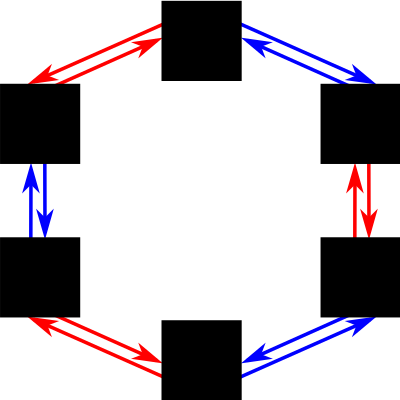
\includegraphics[width=0.8\textwidth]{../../diagrams/hexagon_bi.png}
\end{subfigure}~
\begin{subfigure}[b]{0.45\textwidth}
\vspace{0.5em}
\centering
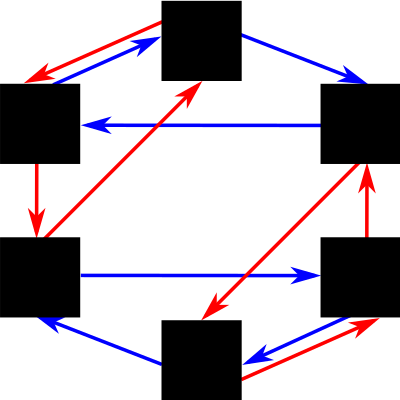
\includegraphics[width=0.8\textwidth]{../../diagrams/hexagon_tri.png}
\end{subfigure}
\end{figure}}
\note{experimental manipulation will be which structure they have in the fractal condition, whether it's the same as door, and outcomes will be performance in fractal condition and abstractions.}
\end{frame}

\againframe<9>{phenomena}

\begin{frame}{Abstractions within task}
Within fractals:
\begin{figure}
\centering
\begin{subfigure}{0.45\textwidth}
\includegraphics[width=\textwidth]{figures/diagram_selection_example.png}
\end{subfigure}~
\begin{subfigure}{0.45\textwidth}
\includegraphics[width=\textwidth]{figures/drag_drop_example.png}
\end{subfigure}
\end{figure}
\end{frame}

\begin{frame}{Abstractions between tasks}
Between tasks:
\begin{figure}
\centering
\begin{subfigure}{0.45\textwidth}
\includegraphics[width=\textwidth]{figures/correspondence_suspect.png}\\
\includegraphics[width=\textwidth]{figures/corr_ident.png}
\end{subfigure}~
\begin{subfigure}{0.45\textwidth}
\includegraphics[width=\textwidth]{figures/corr_drag_drop.png}
\end{subfigure}
\end{figure}
\end{frame}

\section{Results}
\begin{frame}{Subjects in isomorphic condition perform better at task B}
\begin{figure}
\centering
\includegraphics[width=0.9\textwidth]{figures/ex3/ns_more_basic_plot_fractal.png}
\end{figure}
{\scriptsize Error bars represent 95\%-confidence intervals}
\end{frame}

\begin{frame}{Subjects in isomorphic condition perform better at task B}
\begin{figure}
\centering
\includegraphics[width=0.9\textwidth]{figures/ex3/ns_basic_plot_fractal.png}
\end{figure}
{\scriptsize Error bars represent 95\%-confidence intervals}
\end{frame}

\begin{frame}{Subjects in isomorphic condition perform better at task B}
\begin{figure}
\centering
\includegraphics[width=\textwidth]{figures/ex3/ns_stats.png}
\end{figure}
\end{frame}

\begin{frame}{No effect on door performance}
\begin{figure}
\centering
\includegraphics[width=0.9\textwidth]{figures/ex3/ns_basic_plot_door.png}
\end{figure}
{\scriptsize Error bars represent 95\%-confidence intervals}
\end{frame}

\begin{frame}{This may not be conscious}
\begin{figure}
\centering
\includegraphics[width=0.66\textwidth]{figures/ex3/ns_by_correspondence_suspect.png}
\end{figure}
\vspace{-5pt}
{\scriptsize Error bars represent 95\%-confidence intervals}
\end{frame}

\begin{frame}{This may not be conscious}
\begin{figure}
\centering
\includegraphics[width=\textwidth]{figures/ex3/ns_by_cs_stats.png}
\end{figure}
\end{frame}

\begin{frame}{But it may be conscious}
\begin{itemize}
\item Consciousness is tricky to assess \citep{Newell2014}.
    \begin{itemize}
    \item<2-> Can be altered by the exact wording of question or type of probe.
    \end{itemize}
\item<3-> For what it's worth, regressors other than suspecting correspondence give similar results, e.g.:
    \begin{itemize}
    \item<4-> Likert ratings of similarity between the experiments.
    \item<5-> Likert ratings of perception that one task was helpful for the other. 
    \item<6-> Binary split of reports of when they noticed some relationship between the experiments (ever noticed/never noticed).
    \end{itemize}
\end{itemize}
\end{frame}

\begin{frame}[standout]
Evidence of transfer to second task. \par
\uncover<2-> {
May not require consciousness.
}
\end{frame}
\section{Results: Abstractions}

\begin{frame}{Better performance predicts better answers}
\begin{figure}
\centering
\only<1>{
\includegraphics[width=\textwidth]{figures/ex3/ds_by_ns.png}
}
\only<2>{
\includegraphics[width=\textwidth]{figures/ex3/wc_by_ns.png}
}
\end{figure}
\end{frame}

\begin{frame}{Possible future directions}
\begin{itemize}
\item Verify that direction of transfer is caused by order and not e.g. grounding
\item Distractor tasks between
\item Integrating abstractions (either taught or interrogated) earlier on one or both tasks
\item Role of sleep in abstraction
\end{itemize}
\end{frame}

\begin{frame}[allowframebreaks]
\bibliographystyle{plainnat}
\blfootnote{\bibliography{transfer}}
\end{frame}

\appendix

\begin{frame}{Flipping is easier}
\begin{figure}
\centering
\includegraphics[width=0.9\textwidth]{figures/ex3/flipping_easier.png}
\end{figure}
{\scriptsize Error bars represent 95\%-confidence intervals}
\end{frame}

\begin{frame}
\begin{figure}
\centering
\includegraphics[width=0.9\textwidth]{figures/ex3/ns_individual_curve_plot.png}
\end{figure}
{\scriptsize Error bars represent 95\%-confidence intervals}
\end{frame}
\end{document}
